\cleardoublepage

\section{蔗糖酶概论}

蔗糖酶,英文称invertase或sucrase,是一种能够催化蔗糖水解的酶类。该酶首次于1828年由Dumas等在酵母菌发酵蔗糖的过程中被发现,并在1860年由Bertholet首次从酒酵母(Saccharomyces Cerevisiae)中成功分离。系统编号为EC.3.2.1.26,其系统名称为$\beta$-D-呋喃果糖苷果糖水解酶($\beta$-D-fructofuranoside fructohydrolase,$\beta$-D-fructofuranosidase)。

蔗糖酶催化蔗糖非还原末端果糖的$\beta$-D-呋喃果糖苷键水解,生成D-葡萄糖和D-果糖,此反应为不可逆。该酶在植物和微生物中广泛存在,发挥着重要的生理功能。工业上,蔗糖酶被广泛应用,主要来源于酒酵母,以及某些细菌、酵母和丝状真菌,总计超过370种。这些产生的蔗糖酶在理化及生物学特征上与蔗糖酶(EC.3.2.1.26)基本相似。

% 如\autoref{tab:property}所示,
蔗糖酶分为两种类型:外蔗糖酶和内蔗糖酶。外蔗糖酶糖基化达到50\%,位于细胞膜和细胞壁的周质空间,表现出优越的热稳定性和可溶性。相比之下,内蔗糖酶糖基化较低,分布在细胞膜内,含量有限,不适合工业应用。因此,一般所提到的蔗糖酶主要指外蔗糖酶。\cite{kulshrestha2013invertase}

% \begin{table}[H]
% \centering
% \caption{蔗糖酶(EC 3.2.1.26)类型及其性质\cite{gascon1968comparative}}
% \label{tab:property}
% \begin{tabular}{@{}ccc@{}}
% \toprule
% \textbf{类型}  & \textbf{外蔗糖酶}      & \textbf{内蔗糖酶} \\ \midrule
% 存在部位         & 膜壁间隙周质             & 细胞质           \\
% 分子形式         & 同源二聚体              & 同源二聚体         \\
% 单体分子量(KD)    & 110-135            & 65            \\
% 二聚体分子量       & 220-270            & 135           \\
% 糖基化程度        & \textgreater{}50\% & 0-3\%(非糖基化)   \\
% 比活力(unit/mg) & 2700               & 2900          \\
% $K_{m,\mathrm{Sucrose}}$(mM)     & 26                 & 25            \\
% $K_{m,\mathrm{Raffinose}}$(mM)    & 150                & 150           \\
% 等电点pI        & 5.0                & 5.6           \\
% 最适pH         & 3.5-5.5            & 3.5-5.5       \\
% pH稳定性        & 3.0-7.5            & 6.0-9.0       \\
% 最适温度(\dc)      & 60                 & 55            \\ \bottomrule
% \end{tabular}
% \end{table}

蔗糖酶还具有转移酶活性,可利用蔗糖作为转移糖苷的供体和受体合成低聚果糖。然而,在水介质中,其转移酶活性相对较低。高底物浓度或低水介质条件下可提高其转糖基化活性,但由于溶解性或底物抑制问题,使用高底物浓度并不总是可行。此外,\ce{Zn^2+}和\ce{Cu^2+}对蔗糖酶具有较强的抑制作用,而\ce{Ba^2+}、\ce{Mg^2+}和\ce{Mn^2+}略有激活作用。因此,在实验中应注意这些离子对蔗糖酶活性的影响。

如\autoref{fig:mechanism},蔗糖酶催化蔗糖分解的机理可用酸碱催化和共价催化的机理来解释。蔗糖酶在其活性位点结合蔗糖分子,形成酶-底物复合物。在该复合物中,来自酶中的一个羧酸作为通用酸质子化并切断葡萄糖和果糖之间的糖苷键。此后,水分子出作为亲核试剂进攻葡萄糖单元的异头碳,形成半缩醛中间体。去质子的羧酸基团作为通用碱提取水中的一个质子,从而使得葡萄糖单元从酶中解离。此时,果糖单位仍然与酶结合,形成了酶-产物复合物。

此后,水分子作为亲核试剂出现,将其攻击目标对准果糖单位的缩醛碳。这一攻击导致了半缩酮中间体的形成。去质子的羧酸基团再次作为通用碱提取水中的一个质子,从而使得果糖单元从酶中解离。

\begin{figure}[H]
    \centering
    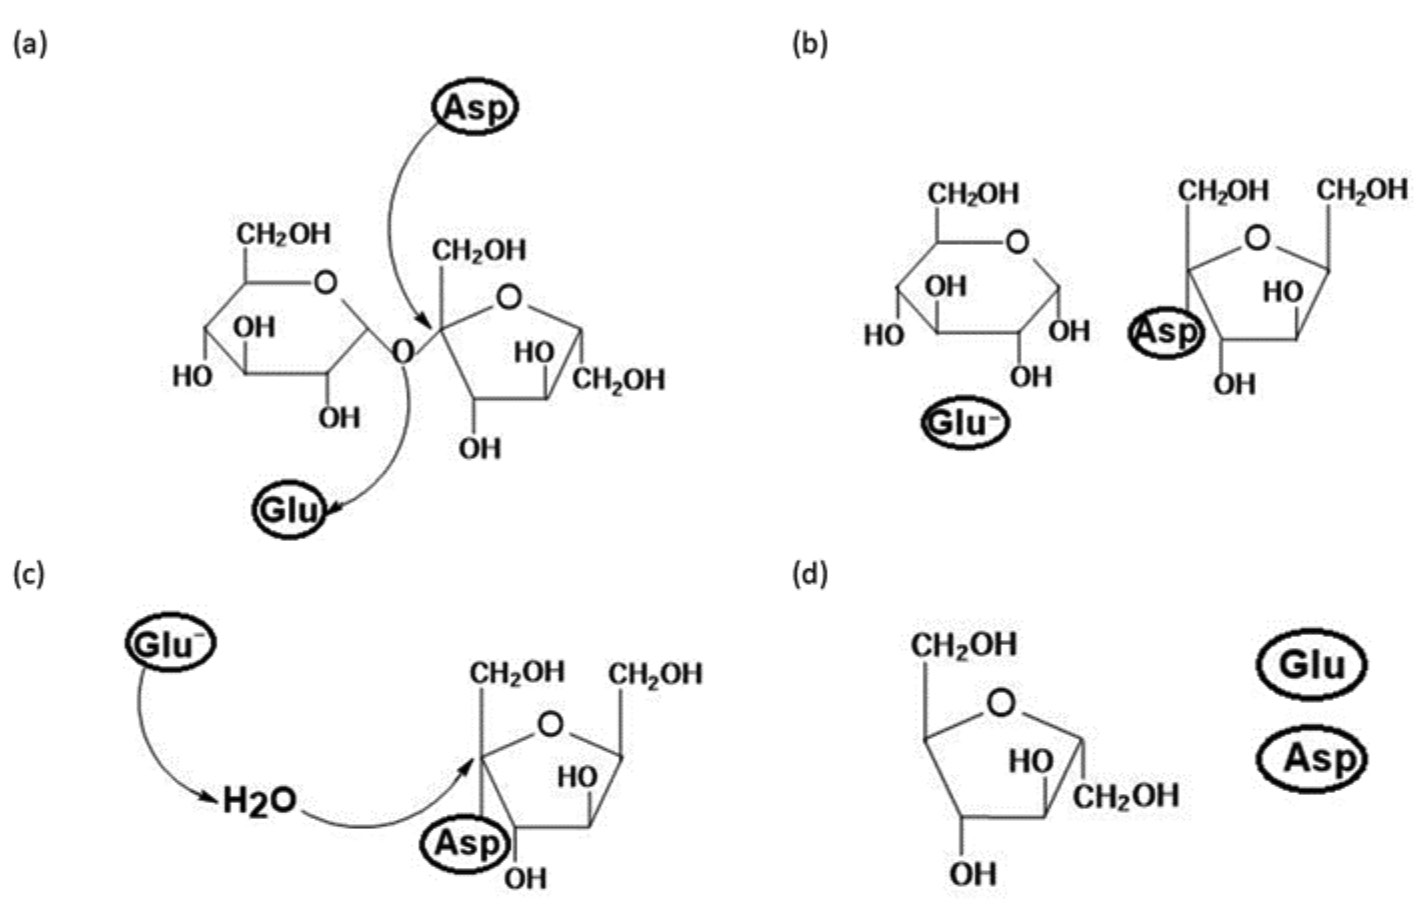
\includegraphics[width = 0.8\textwidth]{figure/principles/mechanism.png}
    \caption{蔗糖酶催化蔗糖分解机理\cite{pang2019structural}}
    \label{fig:mechanism}
\end{figure}